
\documentclass[final,hyperref={pdfpagelabels=false},16pt]{beamer}
\usetheme{Berlin}
\usefonttheme{professionalfonts} % using non standard fonts for beamer
\usefonttheme{serif} % default family is serif

\usepackage[russian]{babel}
\usepackage[utf8]{inputenc}
\usepackage[orientation=portrait,size=a0,scale=1,debug]{beamerposter}
\usepackage
	{
		% Дополнения Американского математического общества (AMS)
		amssymb,
		amsfonts,
		amsmath,
		amsthm,
		physics,
		graphicx
		}
\setbeamertemplate{navigation symbols}{} % минус навигация
\setbeamercolor{block body}{bg=white}
\setbeamerfont{block title}{series=\bfseries}
\let\Tiny=\tiny % решает проблему со шрифтами в TexLive
\setbeamertemplate{headline}{
	\leavevmode
	\begin{beamercolorbox}[wd=\paperwidth]{headline}
		\vspace{2ex}\\
		\begin{columns}[c]
			\begin{column}{.09\paperwidth}
			\end{column}
			\begin{column}{.675\paperwidth}
				\raggedleft
				\usebeamercolor{title in headline}{\textbf{\Huge{\inserttitle}}\\[1ex]}
				\usebeamercolor{author in headline}{\large{\insertauthor}\\[1ex]}
				\usebeamercolor{institute in headline}{\small{\insertinstitute}\\[1ex]}
			\end{column}
			\begin{column}{.25\paperwidth}
				\begin{center}
                    \begin{minipage}{0.49\linewidth}
                        
\includegraphics[width=\textwidth, keepaspectratio]{rf3}
                        
                    \end{minipage}
                    \begin{minipage}{0.49\linewidth}
                        
\includegraphics[width=\textwidth, keepaspectratio]{iap}
                        
                    \end{minipage}

                    \hfill
				\end{center}
			\end{column}
			\begin{column}{.03\paperwidth}
			\end{column}
		\end{columns}
		\vspace{2ex}\\
	\end{beamercolorbox}

 	\begin{beamercolorbox}[wd=\paperwidth]{lower separation line head}
		\rule{0pt}{2pt}
	\end{beamercolorbox}
	\vskip-2cm
	}

\setbeamertemplate{footline}{
	\begin{beamercolorbox}[wd=\paperwidth]{upper separation line foot}
		\rule{0pt}{2pt}
	\end{beamercolorbox}
	\leavevmode%
	\begin{beamercolorbox}[ht=4ex,leftskip=1cm,rightskip=1cm]{author in head/foot}%
		{Оформлено при помощи издательской системы \LaTeX}
        \hfill
		\today
		\hfill
        Github: {github.com/kannab98},   Email: {ponur0kirill@gmail.com}
		\vskip1ex
	\end{beamercolorbox}
	\vskip0pt%
	\begin{beamercolorbox}[wd=\paperwidth]{lower separation line foot}
		\rule{0pt}{2pt}
	\end{beamercolorbox}
	}

\title{Численное моделирование морской поверхности}
\author{Понур К.А.$^{1}$, Караев В.Ю.$^2$, Рябкова М.С.$^2$}
\institute{$^{1}$ Нижегородский Государственный Университет им. М.Ю. Лобачевского \\
          $^2$ Институт Прикладной Физики Российской Академии Наук}
\date{\today}
\newcommand{\tM}{\widetilde{M}}
\usepackage{mathtools}
\mathtoolsset{showonlyrefs}
\begin{document}
  \begin{frame}[t]{} 
    \begin{columns}[t]
      \begin{column}{.48\linewidth}
        \begin{block}{Введение}
            Lorem ipsum dolor sit amet, consetetur sadipscing elitr, sed diam nonumy eirmod
            tempor invidunt ut labore et dolore magna aliquyam erat, sed diam voluptua. At
            vero eos et accusam et justo duo dolores et ea rebum. Stet clita kasd gubergren,
            no sea takimata sanctus est Lorem ipsum dolor sit amet.
        \end{block}
        \begin{block}{Моделирование}
        \begin{equation}
            \zeta(\vec r, t)= \sum\limits_{n=1}^N \sum_{m=1}^M A_n(k_n)\cdot 
            \Phi_{k_nm}(\phi_m) \cos(\omega_n t + \vec k_n \vec r + \psi_{nm}),
        \end{equation}
        Амплитуда, которая является мощностью на интервале $\Delta k_n$, вычисляется по спектру моделируемой поверхности
        \begin{equation}
            A_n(k_n)=\sqrt{ \int\limits_{(\Delta k_n)}  2 S(k) \dd{k}}
        \end{equation}
        $\Phi_{nm}$ -- азимутальное распределение, вычисляемое следующим образом:
        \begin{equation}
        \Phi_{nm}(k_n,\phi_m)=\sqrt{\Phi(k_n,\phi_m) \Delta \phi},
        \end{equation}
        $\Delta \phi$ -- шаг по углу
        
        \begin{figure}[h]
            \centering
            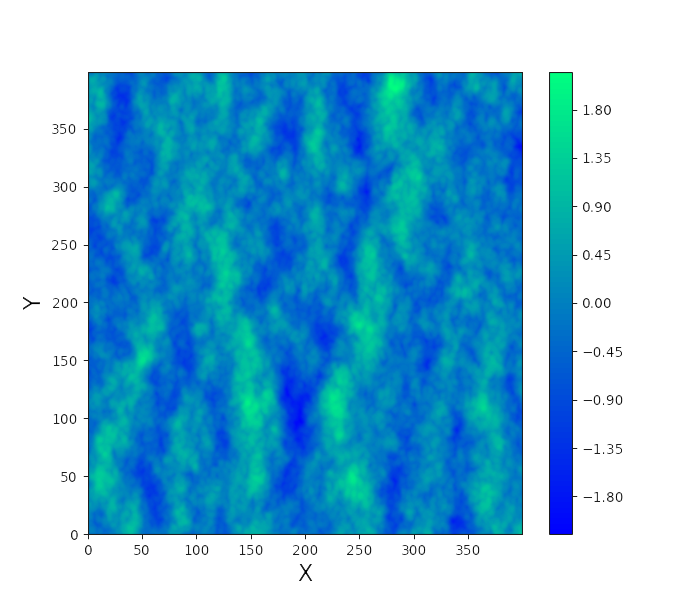
\includegraphics[width=0.6\linewidth]{water10.png}
            \caption{Пример моделируемой поверхности}
            \label{fig:1}
        \end{figure}
        \begin{figure}[h]
            \begin{minipage}{0.32\linewidth}
                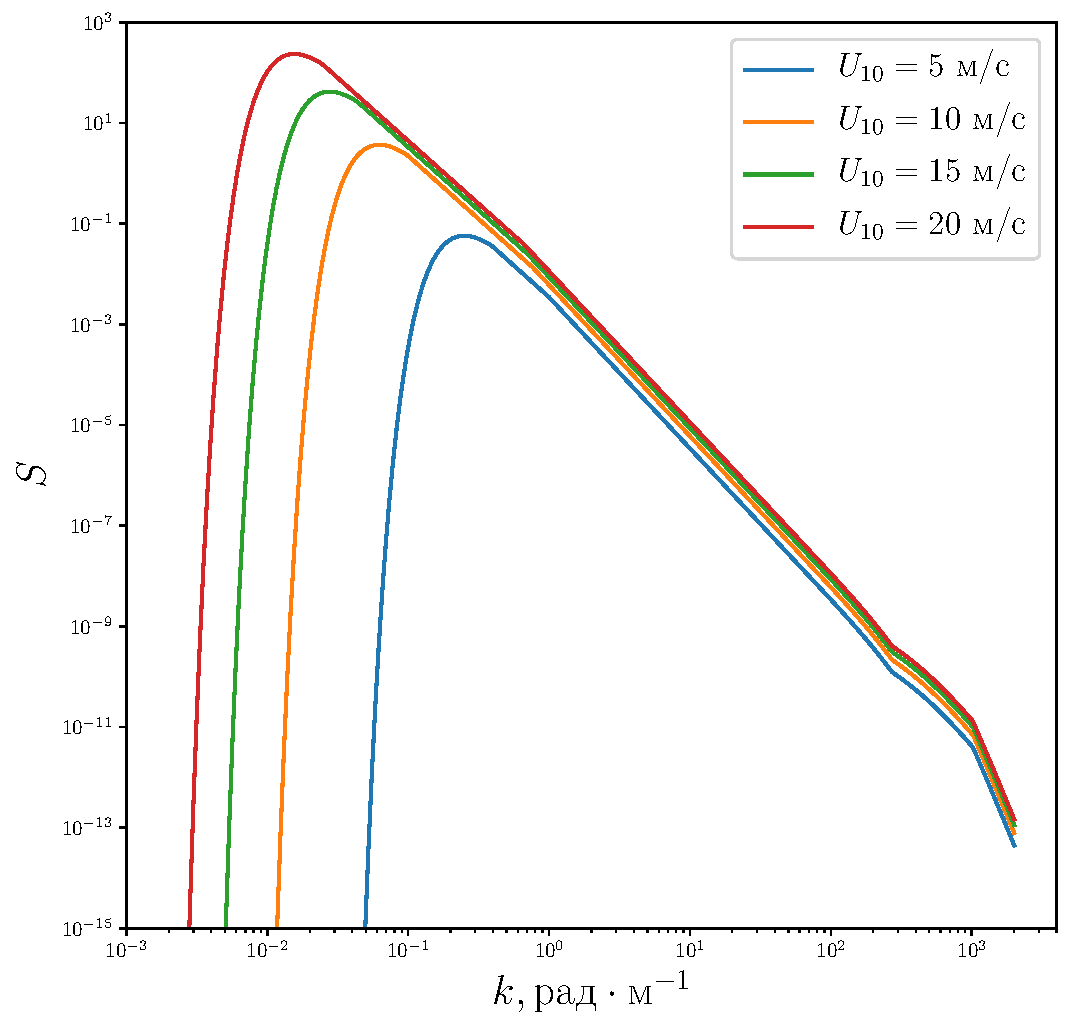
\includegraphics[width=\linewidth]{fig/full_spectrum1}
                \centering
                (a)
            \end{minipage}
            \begin{minipage}{0.32\linewidth}
                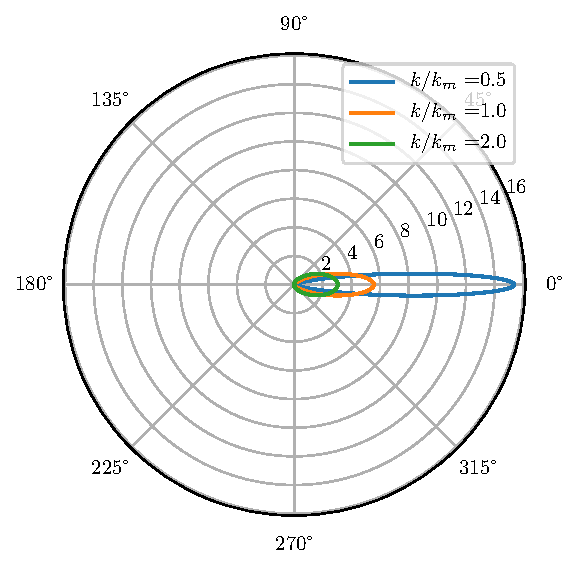
\includegraphics[width=\linewidth]{fig/full_angles1}
                \centering
                (b)
            \end{minipage}
            \begin{minipage}{0.32\linewidth}
                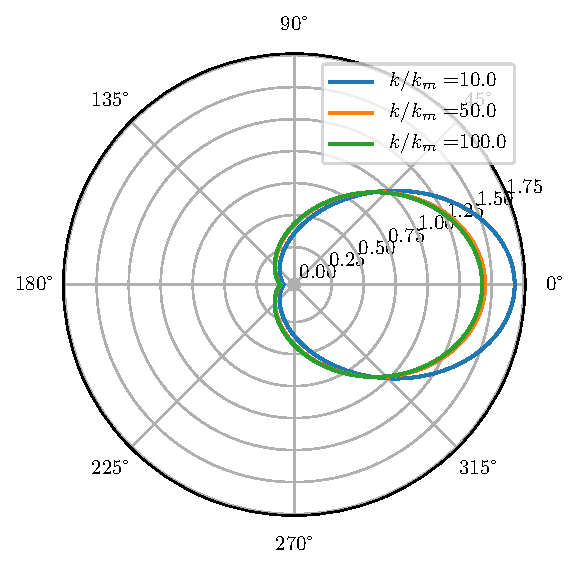
\includegraphics[width=\linewidth]{fig/full_angles2}
                \centering
                (c)
            \end{minipage}
            \caption{Используемый двумерный спектр (a) Зависимость от модуля (b,с) Зависимость от направления}
        \end{figure}
        \end{block}
        \begin{block}{Модель заостренной волны (CWM)}
            Модель заключается в нелинейном преобразовании координат
            \begin{gather}
                x = x_{0} - \sum\limits_{j} \frac{\vec k_j}{\abs{\vec k_j}} \cdot \vec x_{0} \sin(\vec k_j \vec r_{0} - \omega_j t + \phi_j) \\
                y = y_{0} - \sum\limits_{j} \frac{\vec k_j}{\abs{\vec k_j}} \cdot \vec y_{0} \sin(\vec k_j \vec r_{0} - \omega_j t + \phi_j) \\
                z =  \sum\limits_{j=1} a_j \cos(k_j \cdot \vec r_{0} - \omega_j + \phi_j)
            \end{gather}
            Или человеческим языком:
            \begin{equation}
                \label{eq:}
                \qty{\vec r, h(\vec r,t)} \to \qty{\vec r + \vec D(\vec r,t), h(\vec r,t)},
            \end{equation}
            где $\vec r = (x,y)$ -- горизонтальная координата, $D(\vec r,t)$ -- Riesz Transform
            Характеристическая функция такого процесса
            \begin{equation}
                \label{eq:}
                \theta(u) = \qty(1 - i u \sigma_1^2 + u^2 \Sigma_1) \exp{-\frac{1}{2} u^2 \sigma_0^2}
            \end{equation}
            \begin{equation}
                \label{eq:}
                \sigma^2_{\alpha \beta \gamma} = \iint \frac{ \abs{k_x}^{\alpha} \abs{k_y}^{\beta}}{\abs{\vec k}^{\gamma}} \dd{\vec k}
            \end{equation}
        \end{block}
        \begin{block}{Заключение}
            Lorem ipsum dolor sit amet, consetetur sadipscing elitr, sed diam nonumy eirmod
            tempor invidunt ut labore et dolore magna aliquyam erat, sed diam voluptua. At
            vero eos et accusam et justo duo dolores et ea rebum. Stet clita kasd gubergren
            no sea takimata sanctus est Lorem ipsum dolor sit amet.
        \end{block}
        \begin{block}{Литература}
            \footnotesize
            \begin{thebibliography}{}
                \bibitem{Rytov} \textit{С.М. Рытов}, Введение в статистическую радиофизику // Изд. 2-е, перераб. и доп. - Москва : Наука, 1976. - Ч. 1. Случайные процессы \S\S 14-18, 38-42 
                \bibitem{Karaev1} \textit{В.Ю.Караев, М.Б. Каневский, Г.Н. Баландина}, Численное моделирование поверхностного волнения и дистанционное зондирование // Препринт №552 ИПФ РАН, 2002, С.1-10.
                \bibitem{Veber} \textit{В.Л. Вебер}, О моделировании случайного профиля морской поверхности // Изв. вузов. Радиофизика. 2017. Т. 60, № 4. С. 346.
                \bibitem{Karaev2} \textit{В.Ю.Караев, Г.Н. Баландина} Модифицированный спектр волнения и дистанционное зондирование // Исследование Земли из космоса, 2000, N5, C.1-12.
                \bibitem{Longe} \textit{М.С. Лонге-Хиггинс} Статистический анализ случайной движущейся поверхности // в кн.: Ветровые волны, М.: Иностранная наука, 1962, С.112-230
            \end{thebibliography}
        \end{block}
      \end{column}
      \begin{column}{.48\linewidth}
        \begin{block}{Метод <<отбеливания>> спектра}
            Предположим, что гармонические составляющие при больших $\rho$ складываются <<некогерентным>> образом. То есть  мощность шума определяется как
            \begin{equation}
                \sigma^2_{\text{шум}}= \sum_{i=1}^N \frac{b_i^2}{2}
            \end{equation}
            В области малых $\rho$ гармоники суммируются <<когерентно>> и соответствующая мощность равна
            \begin{equation}
                \tM^2(0)=\qty(\sum_{i=1}^N b_i)^2
            \end{equation}
            Введем функцию, характеризующую относительную мощность шумов
            \begin{equation}
                \label{eq:Q}
                Q = \frac{\sigma^2_{\text{шум}}}{\tM^2(0)}
            \end{equation}
            Минимизируем величину \eqref{eq:Q}, решая систему уравнений
            \begin{equation}
                \label{eq:cases}
                \pdv{Q}{b_i}=\frac{b_i}{\qty (\sum\limits_{i=1}^{N} b_i)^2} - \frac{\sum\limits_{i=1}^{N} b_i^2}{\qty (\sum\limits_{i=1}^{N} b_i)^3}, ~ i = 1\hdots N.
            \end{equation}
            Она сводится к следующей системе:  $b_i \sum\limits_{i=1}^{N} b_i -\sum\limits_{i=1}^{N} b_i^2=0 $
             \vfill
            Частным результатом решения является $b_1=b_2=\hdots=b_N$.
            \vfill
    % Задача сводится к разбиению области определения спектра на участки $\Delta k_i$, интегралы по которым от функции $S(k)$ имеют одинаковые значения.

           \begin{equation}
                \text{Для высот:}\quad 	b_i=b_1= \frac{M(0)}{N}=\frac1N \int\limits_0^{\infty} S(k) \dd{k}
           \end{equation}
           \begin{equation}
                \text{Для наклонов:}\quad 	b^{\theta}_i=b^{\theta}_1= \frac{M^{\theta}(0)}{N}=\frac1N \int\limits_0^{\infty} k^2S(k) \dd{k}
           \end{equation}
            Потребуем сопряжения в нуле всех производных  функций
            $\tM(\rho)$ и $M(\rho)$. 
            Для функции корреляции стационарной случайной функции $M(\rho)$ справедливо
            \begin{equation}
                M'_{\rho}=\pdv[2]{M(\rho)}{\rho}=\int\limits_{0}^{\infty} k^2 S(k)\cos(k \rho)\dd{k}
            \end{equation}
            А значит можно переписать наше требование в виде
            \begin{equation}
                \sum_{i=1}^N b_ik_i^{2p}=\int\limits_{0}^{\infty} k^{2p}S(k)\dd{k}, p = 1,2,\dots,N.
            \end{equation}
            Решать такую систему довольно сложно, поэтому потребуем выполнение более простого равенства
            \begin{equation}
                \sum_{i=1}^N b_ik_i^{2}=\int\limits_{0}^{\infty} k^{2}S(k)\dd{k}
            \end{equation}
            \begin{minipage}{0.49\linewidth}
                \centering Для наклонов:
                \begin{equation}
                    k_i=\sqrt\frac{N}{{\int\limits_{0}^{\infty} k^2 S(k) \dd{k}}}\cdot {\int\limits_{\Delta k_i} k^4 S(k) \dd{k}}
                \end{equation}
                \end{minipage}
                \hfill
                \begin{minipage}{0.49\linewidth}
                \centering Для высот:
                \begin{equation}
                    k_i=\sqrt\frac{N}{{\int\limits_{0}^{\infty} S(k) \dd{k}}}\cdot \int\limits_{\Delta k_i} k^2 S(k) \dd{k}
                \end{equation}
                \end{minipage}
                \vfill
                Решением будем считать суперпозицию решения системы уравнений
                \eqref{eq:cases} для высот и наклонов
                \begin{figure}[H]
                    \begin{minipage}{0.49\linewidth}
                            \centering
                            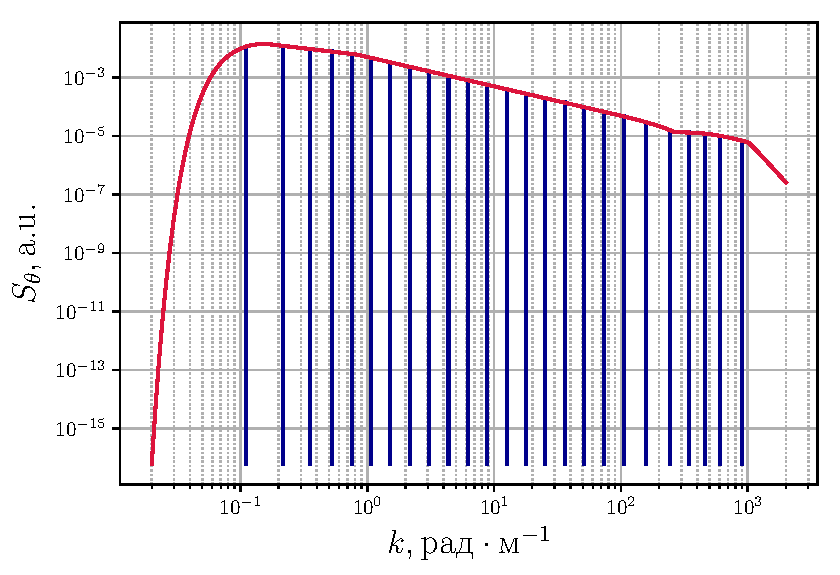
\includegraphics[width=\linewidth]{fig/split_angles}	
                    \end{minipage}
                    \hfill
                    \begin{minipage}{0.49\linewidth}
                            \centering
                            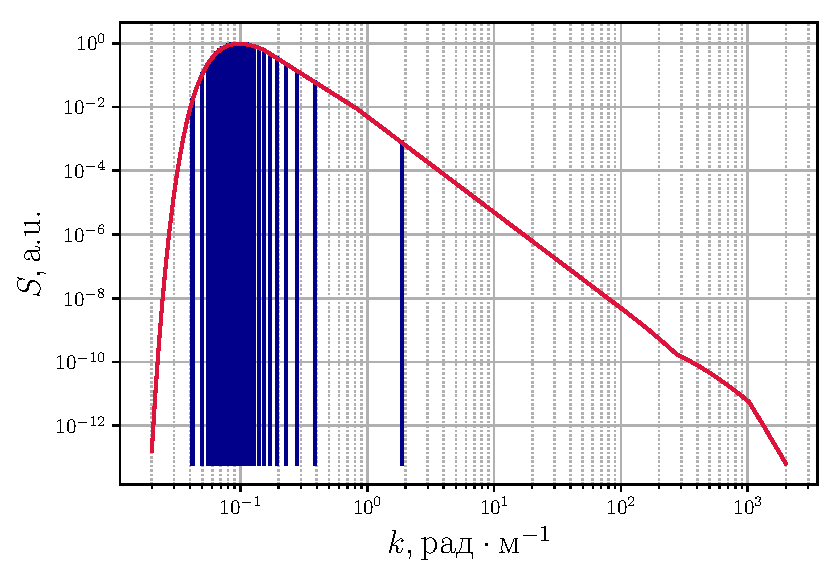
\includegraphics[width=\linewidth]{fig/split_height}
                    \end{minipage}
                    \caption{Расположении узлов по методу <<отбеливания>> спектра  для наклонов и высот соответственно. $U=10 \frac{\text{м}}{c}$, $N=25$}
                    \label{fig:splits}		
                \end{figure}
        \end{block}
      \end{column}
    \end{columns}
  \end{frame}
\end{document}
